
%(BEGIN_QUESTION)
% Copyright 2014, Tony R. Kuphaldt, released under the Creative Commons Attribution License (v 1.0)
% This means you may do almost anything with this work of mine, so long as you give me proper credit

Set up a current transformer, a set of multimeters, and an adjustable AC power supply to perform a saturation test on a current transformer.  If your adjustable AC power supply cannot produce a voltage equal to or greater than the ``class'' rating of the CT (e.g. at least 200 volts to test a C200 current transformer), you may be able to perform a similar test using a high-{\it current} AC such as a protective relay test to drive current through the primary of the CT:

$$\includegraphics[width=15.5cm]{i03087x01.eps}$$

Identify the relevant data you will need to collect in this experiment to determine the CT's saturation point (i.e. the ``knee point'' voltage).  Use a computer spreadsheet if you wish to plot this data and show it in graphical form.

\vskip 10pt

Lastly, determine a test by which you could determine the {\it polarity} of the CT, supposing it is not already marked.

\underbar{file i03087}
%(END_QUESTION)





%(BEGIN_ANSWER)

The {\it Lessons In Industrial Instrumentation} textbook shows how this is done, and provides a sample table of data from a real-life CT rat/sat test.

%(END_ANSWER)





%(BEGIN_NOTES)

Blue Sea Systems makes a tiny little CT (rated 50 A primary and 50 mA secondary for a 1000:1 ratio) with a part number of 9633 which saturates beautifully when performing a primary injection test.  The 1000:1 ratio makes it easy to measure a strong voltage with just a small amount of input current (less than 5 amps AC on the primary with an open-circuited secondary).  Here is some data taken from such a Blue Sea Systems CT, along with some random CT (``mystery'') I found in my collection:

$$
\includegraphics[width=15.5cm]{i03087x02.eps}$$

%INDEX% Electronics review: current transformer (CT)

%(END_NOTES)


